%% ===========================================================================
%% A reproducible IPPU accounting platform for Pakistan
%% Target journal: Environmental Modelling & Software (Elsevier)
%% ===========================================================================
\documentclass[5p,times,authoryear]{elsarticle}
% ===========================================================================
% Shared preamble for every manuscript in this repository.
%
% Papers using it:
%   paper/            agriculture inventory
%   paper_nowcast/    agricultural nowcasting
%   paper_national/   the nine-sector national inventory
%   notes/<sector>/   one data note per non-agriculture sector
%
% It exists because paper/ and paper_nowcast/ began as copies of one another
% and had already drifted five lines apart before a third manuscript existed.
% Eleven copies would drift eleven ways, and a macro that renders differently
% in two papers is the kind of defect nobody notices until proof stage.
%
% \graphicspath is deliberately NOT set here - each manuscript sets its own
% after \input{...preamble}, because figures live beside the document.
% ===========================================================================

\usepackage[utf8]{inputenc}
\usepackage[T1]{fontenc}
\usepackage{amsmath,amssymb}
\usepackage{graphicx}
\usepackage{booktabs}
\usepackage{multirow}
\usepackage{siunitx}
\usepackage[colorlinks=true,citecolor=blue,linkcolor=blue,urlcolor=blue]{hyperref}
% Document-information metadata for every PDF in the bundle (the seventh review noted
% the shipped PDFs carried none). Documents that set their own \hypersetup{pdftitle=...}
% keep it - hyperref takes the LAST setting, and this shared block runs first. Full
% tagged-PDF (tagpdf / \DocumentMetadata) is deliberately not attempted here: the
% installed LaTeX toolchain's support is not uniform across sixteen documents, and a
% half-tagged bundle is worse than an honestly untagged one; deferred deliberately.
\hypersetup{
  pdfauthor={Rehan Ahmad, Pakistan Air Quality Initiative (PAQI)},
  pdfsubject={A reproducible ten-sector national greenhouse-gas inventory
              for Pakistan},
  pdfkeywords={Pakistan, greenhouse gas inventory, IPCC 2006 Guidelines, MRV,
               reproducible research, emissions, air pollutants},
}
\usepackage{caption}
\captionsetup[table]{position=below}
\usepackage{enumitem}
\usepackage{xcolor}
\usepackage{float}
\usepackage{placeins}
\usepackage{tabularx}
\usepackage{natbib}
\usepackage{tikz}
\usetikzlibrary{arrows.meta,positioning,fit,backgrounds}

\setlength{\emergencystretch}{3em}

% Looser float placement to prevent pile-up in two-column mode.
\renewcommand{\topfraction}{0.95}
\renewcommand{\bottomfraction}{0.85}
\renewcommand{\textfraction}{0.05}
\renewcommand{\floatpagefraction}{0.85}
\setcounter{topnumber}{4}
\setcounter{bottomnumber}{3}
\setcounter{totalnumber}{6}

% ---------------------------------------------------------------------------
% Custom shorthand: in macros.tex since the ESSD re-targeting, because the national
% article compiles under the Copernicus class and cannot take this preamble (the class
% loads its own packages) but needs exactly the same macros. This file inputs it so that
% every other manuscript keeps compiling unchanged.
%
% THREE relative paths, because \input resolves against the COMPILE DIRECTORY and not
% against this file, so the depth is a property of whoever is building:
%   ../paper_common      a manuscript compiled from one level down
%   ../../paper_common   papers/<sector>/ and notes/<sector>/
%   ../../../paper_common  paper_national/versions/<v>/, since the national paper was
%                          versioned - that move is what added this third arm, and the
%                          supplement failed with "../../paper_common/macros.tex not
%                          found" until it was here
% A fourth depth needs a fourth arm, which is the cost of keeping a bare `latexmk` in a
% manuscript directory working without a TEXINPUTS set for it.
% ---------------------------------------------------------------------------
\IfFileExists{../paper_common/macros.tex}%
  {\input{../paper_common/macros}}%
  {\IfFileExists{../../paper_common/macros.tex}%
    {% ===========================================================================
% paper_common/macros.tex - the shorthand every manuscript shares.
%
% Split from preamble.tex in the ESSD re-targeting: the national article now compiles
% under the Copernicus class, which loads its own packages and forbids most of what
% preamble.tex sets (geometry-like options, a second hyperref, placeins), but it needs
% exactly the same shorthand as the sector reports. The macros therefore live here, on
% their own, and preamble.tex inputs this file so that every other manuscript keeps
% compiling unchanged. A macro that renders differently in two documents is the defect
% this file exists to prevent; define it once.
%
% Requires: siunitx (for \DeclareSIUnit and \si) - the caller loads it.
% ===========================================================================

% Gas and pollutant names.
\newcommand{\COtwo}{CO\textsubscript{2}}
\newcommand{\COe}{CO\textsubscript{2}e}
\newcommand{\CHfour}{CH\textsubscript{4}}
\newcommand{\NtwoO}{N\textsubscript{2}O}
\newcommand{\NHthree}{NH\textsubscript{3}}
\newcommand{\NOx}{NO\textsubscript{x}}
\newcommand{\SOtwo}{SO\textsubscript{2}}
\newcommand{\PM}{PM\textsubscript{2.5}}
\newcommand{\MCF}{MCF}
\newcommand{\Mt}{\text{Mt~\COe}}
\newcommand{\tCha}{\si{\tonne\per\hectare}}
\newcommand{\AFOLU}{AFOLU}
\newcommand{\GLW}{GLW\,4}
\newcommand{\EFone}{EF\textsubscript{1}}

% siunitx: allow Mt, Tg, ha, head, yr, dB
\DeclareSIUnit{\head}{head}
\DeclareSIUnit{\yr}{yr}
\DeclareSIUnit{\dB}{dB}

% A file name is the one long unbreakable token these documents are full of -
% \texttt{waste\_air\_pollutants\_2024.csv} is wider than a two-column measure and TeX prints
% it past the margin rather than breaking it. Allowing a break AFTER each escaped underscore
% costs nothing and inserts no hyphen, which matters: a hyphenated file name is a wrong file
% name. This is one line because every such name in every document is written with \_.
\let\pkinvunderscore\_
\renewcommand{\_}{\pkinvunderscore\allowbreak}
}%
    {\input{../../../paper_common/macros}}}
% Long unbreakable strings - output filenames, module paths, URLs in \texttt - do not fit a
% two-column measure and TeX prints them past the margin rather than breaking them. Nothing
% read the log, so 47 of those overruns shipped across seven documents. Emergency stretch lets
% the paragraph loosen instead, and \texttt is taught to break at the punctuation these names
% actually contain.
\emergencystretch=6em


\graphicspath{{figures/}}
\journal{Environmental Modelling \& Software}
\begin{document}
\begin{frontmatter}
\title{PakEmis Sector Technical Note TN07\\[4pt]
An Evidence-Gated IPPU Accounting Framework for Pakistan: A Cement (2.A.1) Module Estimated, Every Other Category's Requirements Documented}
\author[paqi]{Rehan Ahmad\corref{cor1}}
\ead{rehan@pakairquality.com}
\address[paqi]{Pakistan Air Quality Initiative (PAQI), Karachi, Pakistan}
\cortext[cor1]{Corresponding author}
\begin{abstract}
Pakistan's industrial-process activity data are distributed across manufacturing statistics,
trade records, company reports, product-use data and national greenhouse-gas reporting. We
develop a reproducible Industrial Processes and Product Use (IPPU) framework that links each
IPCC category to process-specific activity data and material balances. Categories lacking
sufficient evidence remain explicitly unestimated, with their data requirements documented.
The reference GHG module estimates cement calcination, ammonia production net of recovered carbon, iron and steel, and lubricant use. Its FY2023--24 total is \SI{25.535}{\mega\tonne} CO$_2$; categories lacking supported methods and activity remain unestimated. The accompanying air product has its own admitted process coverage, including ammonia, steel and soda ash; this does not turn every IPPU GHG omission into an estimate.

A source-period audit shows that \SI{48.011}{\mega\tonne} of cement previously attributed to
FY2023--24 corresponds to FY2021--22; PBS and State Bank statistics both report
\SI{39.566}{\mega\tonne} for FY2023--24. Accounting for \SI{3.792}{\mega\tonne} of
clinker exports and \SI{0.026}{\mega\tonne} of imports gives
\SI{33.440}{\mega\tonne} of inferred domestic clinker production. That Tier~1 inference
gives a cement process estimate of 17.389--21.504 Mt \COtwo{} across the IPCC
clinker fractions of 0.75 and 0.95, both ends priced as named national configurations.
The reference is neither end: it is the clinker the producers themselves report.

All sixteen producer filings independently report \SI{41.953}{\mega\tonne} of clinker,
125.5\% of the low-clinker Tier~1 inference and 101.4\% of the high case, which at the
common factor gives the reference \SI{21.816}{\mega\tonne} \COtwo{} (conditional 95\%
interval 20.227--23.452 Mt); the 0.75-fraction model is priced beside it as the national
configuration \emph{cement\_tier1\_model\_low}. The gap between the census and the
high-clinker inference indicates unresolved differences in reporting coverage, clinker
transfers and stock movements rather than a small residual activity gap. A matched calendar-2022
reconstruction gives 17.985--22.595 Mt \COtwo{}, compared with
\SI{27.906}{\mega\tonne} in Pakistan's official cement inventory. The full official IPPU
inventory is \SI{49.112}{\mega\tonne} \COe{}, including 19.400 Mt from chemical
industries.

These results show that clinker trade and reporting-period alignment materially affect cement
estimates, while company production data can potentially replace Tier~1 clinker assumptions.
The national annual core now covers July 2015--June 2025. This note retains the detailed FY2023--24 clinker and reporting comparisons. Plant-specific ammonia recovery, nitric-acid abatement and fluorinated-gas equipment data remain consequential limitations.

\end{abstract}
\begin{keyword}
industrial processes \sep IPPU \sep clinker trade \sep material-flow accounting \sep
F-gases \sep completeness \sep uncertainty \sep Pakistan
\end{keyword}
\end{frontmatter}

%% Generated by scripts/make_release_cover.py; says which release this documents.
% The Sector Technical Note banner (v1.0.0). Each sector manuscript is a PakEmis Sector
% Technical Note, numbered TN01-TN10 in src/pkinv/release.py (TECHNICAL_NOTES), and says
% so on its first page: it documents ONE sector module of the release named in the block
% that follows, and the national totals are stated only in the data-description article
% (the cover block below reproduces them as release identity, not as a claim of this note).
% Usage, in the document body before the release cover:  \TNBanner{TN01}
\providecommand{\TNBanner}[1]{%
  \noindent\fbox{\parbox{\dimexpr\linewidth-2\fboxsep-2\fboxrule}{%
    \textbf{PakEmis Sector Technical Note #1.} Technical documentation of one sector
    module of the PakEmis release identified below, deposited with the data as part of the
    documentation record. The national data-description article (\texttt{paper\_national/})
    is the only document that states the national totals as its own result.%
    \InputIfFileExists{../../paper_common/generated_availability_tn}{}{}%
  }}\par\medskip}

\TNBanner{TN07}
%% GENERATED by scripts/make_release_cover.py from outputs/release_manifest.json.
%% Do not edit: the edit will be overwritten and CI diffs the result.
\newcommand{\ReleaseCover}{%
\begin{center}\small
\setlength{\fboxsep}{4pt}%
\fbox{\begin{minipage}{\dimexpr\linewidth-2\fboxsep-2\fboxrule\relax}\footnotesize
\textbf{Release provenance.} This document describes PakEmis under the period, configuration and source boundaries specified in its methods. The identifiers below link it to the accompanying products and source register.\\[2pt]
\begin{tabular}{@{}p{0.32\linewidth}@{\hspace{0.03\linewidth}}p{0.65\linewidth}@{}}
Release version & \texttt{1.0.0rc69} \\
Commit & \texttt{d8d874622f9a} \\
Reporting period & July 2015--June 2025 (ten fiscal years) (2015-07-01 to 2025-06-30) \\
Reference & S\_TAN (household survey; TAN nitrogen) \\
FY2023--24 total & 444.61 Mt \COe{} (AR5) under S\_TAN, the reference; 449.85 Mt under L\_TAN \\
Release manifest & \texttt{ac0ffe93ad9fcd88} (SHA-256 of \texttt{outputs/release\_manifest.json}, first 16) \\
Source manifest & \texttt{c1be6d314cfce1ea} (SHA-256 of \texttt{data/manifests/source\_manifest.csv}, first 16) \\
Data-description article & \texttt{paper\_national/} (ESSD, in preparation), same release
\end{tabular}
\end{minipage}}
\end{center}}

\ReleaseCover

\section{Introduction}
\label{sec:intro}

Industrial Processes and Product Use (IPPU) is not one calculation. It includes carbonate
decomposition in cement, lime and glass; feedstock carbon in ammonia and petrochemicals;
nitrous oxide from nitric acid; carbon inputs to metals; non-energy uses of fuels; and
fluorinated gases held in equipment and products \citep{ipcc2006ippu,ipcc2019}. These sources
share an inventory sector but not an activity unit, emission factor or spatial representation.
A credible national account must therefore do two things at once: connect each process to its
own physical activity and identify explicitly which categories remain unestimated because
process-specific activity data are insufficient.

Earlier work independently estimated cement calcination from one cement statistic, one
assumed clinker fraction and one emission factor, but did not yet provide a sector-wide IPPU
framework. It also omitted a required term in the cement method. When clinker production is inferred from cement,
IPCC's Tier~1 worksheet requires clinker imports and exports because calcination emissions
occur where clinker is produced rather than where it is ground or consumed. Pakistan is a
substantial net clinker exporter, so that correction is material.

This study asks one question: \emph{how far can a reproducible, physically coherent IPPU
inventory be built from currently public Pakistani evidence while restricting emission
estimates to categories for which the relevant process-specific activity data are available?}

We address three questions. First, what does a correct period- and trade-matched public-data
calculation imply for cement calcination? Second, how closely does inferred national clinker
agree with company-reported production, and which evidence still prevents a complete Tier~2
balance? Third, what does Pakistan's official reporting imply about the material categories
that remain outside the independent estimate? We answer them by reconciling cement production
and trade in a material balance, comparing inferred clinker with producer filings, auditing
the CRT at cell level and assessing data completeness across 2.A--2.G.

The analysis establishes both an estimate and the present limits of the available evidence.
Cement 2.A.1 is estimated for FY2023--24 and reconstructed independently for calendar 2022.
Public data identify glass, soda ash, steel products, lubricants, HFC consumption and partial
ammonia/nitric-acid activity, but estimating their emissions requires additional evidence on
process routes, recovery, abatement or equipment stocks.

\section{Accounting Context}
\label{sec:related}

\subsection{A heterogeneous inventory sector}

IPCC Volume~3 organises IPPU into mineral industries (2.A), chemical industries (2.B),
metal industries (2.C), non-energy products from fuels and solvents (2.D), electronics
(2.E), fluorinated substitutes for ozone-depleting substances (2.F), and other product
manufacture and use (2.G) \citep{ipcc2006ippu}. The 2019 Refinement updates important methods
and factors but does not remove the central data requirement: the activity must correspond to
the physical process that emits.

This is why headline production quantities can be misleading. Cement output is not clinker
production. Total fertiliser output differs from ammonia production. Billets do not identify
the steelmaking route or its carbon inputs, and annual HFC leakage depends on the applications
and equipment stocks in which the chemicals are used. Each quantity is valuable evidence, but
the relevant process definition is also required.

\subsection{Material balances as shared accounting}

Several IPPU categories become clearer when written as conserved material flows. For cement,
domestic clinker production plus imports minus exports and stock accumulation must equal the
clinker ground into cement. For ammonia, feedstock carbon becomes gross process \COtwo{}, which
is divided among atmospheric emissions, urea production, other recovery and any permanent
storage. For fluorinated gases, annual supply enters equipment banks and leaves through
manufacturing losses, operating leakage, retirement, recovery and destruction.

These balances complement IPCC emission factors by constraining the activity bases to
which those factors apply and expose residuals that a collection of independent equations can
hide. They also connect IPPU to neighbouring sectors without double counting: cement kiln
fuel remains Energy 1.A.2, while clinker calcination remains IPPU 2.A.1.

\subsection{Evaluation and official reporting}

Broad global products such as EDGAR are useful only after year, category, gas and GWP are
matched. A national ``Processes'' total cannot validate cement alone. Pakistan's own CRT is a
stronger accounting comparator because it exposes category rows, native gases, activity data,
implied factors, recovery and notation keys \citep{pakcrt2026}. We therefore use the CRT as an
official method audit and scope comparator. Public production, trade and consumption datasets
provide separate evidence for activity magnitude and reporting boundaries.

\section{Data and Evidence Roles}
\label{sec:data}

\subsection{Cement activity and its period audit}

The official PBS Quantum Index of Manufacturing (QIM) reports
\SI{39.566}{\mega\tonne} of cement output for FY2023--24 \citep{pbsqim2024}. The State
Bank's FY2023--24 Statistical Supplement independently reproduces that value and provides a
five-year fiscal series \citep{sbpstatsupp2024}: 39.121, 49.797, 48.011, 41.448 and
39.566 Mt for FY2019--20 through FY2023--24. This establishes that the
\SI{48.011}{\mega\tonne} value previously attributed to FY2023--24 belongs to FY2021--22.
It is retained as a historical benchmark rather than a current structural alternative.

The annual core extends from FY2015--16 through FY2024--25 using held fiscal physical-production and trade records. The detailed reference-year analysis below remains FY2023--24. Publication revisions and source vintages are retained rather than interpreted as competing observations for one unchanged boundary.

QIM also reports FY2023--24 production of soda ash (\SI{0.785}{\mega\tonne}), billets and
ingots (\SI{4.914}{\mega\tonne}), glass plates and sheets
(\SI{20.205e6}{\metre\squared}) and lubricating oil
(\SI{130.513e6}{\litre}). These statistics establish the occurrence and scale of the
activities but do not provide every variable required by IPCC.
Glass needs mass, type, cullet and carbonate inputs; steel needs the production route and
carbon inputs; lubricants require non-energy consumption and oxidation rather than output.

Monthly UN Comtrade records for HS~252310 were summed from July 2023 through June 2024
\citep{uncomtrade2024clinker}. Exports total \SI{3.792074}{\mega\tonne} and imports
\SI{0.026131}{\mega\tonne}, with all twelve months present for both flows.

The panel now extends back to July 2014 for both flows, and every fiscal year of the
national series resolves to an observed trade term. Extending it required deciding what an
EMPTY month means, because the source returns no record both for a month in which nothing
was traded and for a month it has not processed, and the response does not distinguish
them. Pakistan's clinker imports are small and sporadic---\SI{0.026131}{\mega\tonne}
across the whole of FY2023--24 against \SI{3.792074}{\mega\tonne} exported---so empty
months are
common, and reading them as zeros would manufacture a complete panel from an incomplete
one, in the direction that lowers inferred domestic production. Each calendar year's
annual-frequency total was therefore retrieved as a control: a month with no record counts
as zero only where the monthly records of its calendar year already sum to that year's
annual total, so the source itself certifies that nothing further moved. Where they do not
sum, the month is unobtained and the fiscal years touching it are NE. Months lacking a record count as zero only after this compatible source-control check; unresolved coverage remains explicit. The
per-year verdicts are generated by \texttt{pkinv.sectors.ippu.trade\_evidence}. For the official
comparison year, January--June 2022 QIM observations were joined to July--December 2022 and
sum to \SI{44.331}{\mega\tonne}. Calendar-2022 WITS/UN Comtrade records give
\SI{1.341580}{\mega\tonne} of exports and \SI{0.003999}{\mega\tonne} of imports
\citep{witsclinker2022}.

\subsection{Producer and facility evidence}

We identified 16 cement producers relevant to FY2023--24. All sixteen public filings disclose
\SI{41.953170}{\mega\tonne} of clinker production
\citep{luckycement2024,dgkcement2024,attockcement2024,powercement2024,
cheratcement2024,pioneercement2024,thattacement2024,bestwaycement2024,
kohatcement2024,dandotcement2024,gharibwalcement2024,dewancement2025,
faujicement2024,mapleleafcement2024,flyingcement2024}.
Where disclosed, we also compiled opening and closing stocks, clinker purchases and imports,
clinker ground, domestic sales and exports. Missing flow terms remain unobserved, so company
balances are evaluated only where the necessary data are available.

Flying's scanned annual report gives exact FY2023--24 clinker and cement production of
\SI{0.322624}{\mega\tonne} and \SI{0.321500}{\mega\tonne}, respectively; Fecto's FY2025
annual report states the FY2023--24 comparative directly, \SI{0.651048}{\mega\tonne} of
clinker and \SI{0.724209}{\mega\tonne} of cement, where its earlier public briefing had
given only capacity and rounded utilisation
\citep{fectocement2024,fectocement2025,flyingcement2024}. All \num{16} census companies
therefore report an exact clinker quantity; what no company reports is the balance
around it (purchases, sales, grinding and stocks). The census is
\texttt{ippu\_cement\_producer\_census\_2024.csv}.

The facility registry identifies cement and fertiliser installations by operator, process route and administrative area. Coordinate provenance is retained for each record. The primary geographic package uses only locations compatible with its declared licence, while ODbL-derived locations retain a separate alternative. Company-wide clinker is split conditionally among works where plant-specific output is unavailable; unsupported placement remains unallocated. A point location does not itself establish plant production.

\subsection{Official reporting, chemicals and product-use data}

Pakistan's 2024 CRT submission contains a dedicated workbook for inventory year 2022
\citep{pakcrt2026}. We preserve ZIP and workbook hashes, worksheet names, cell addresses, raw
values and formulas. Table~2(I) provides category emissions; Table~2(I).A--H provides
activity, implied factors, native gases and recovery; and Table~2(II).B--Hs2 provides
species-level F-gas records.

Public company reports provide initial evidence for the next categories. Fatima
reports \SI{0.311242}{\mega\tonne} of calendar-2024 ammonia production at Sheikhupura; historical
records identify ammonia and nitric-acid output at Sadiqabad, dual-pressure nitric-acid
technology and CDM abatement projects at Sadiqabad and Pakarab \citep{fatima2024,pakarabcdm,
fatimacdm}. The NFDC annual review adds four extracted tables: domestic fertiliser production
by product and manufacturer, product-wise offtake split domestic and imported, plant-wise
fertiliser-sector gas, and the same gas monthly by plant for both fiscal years. The
feedstock/fuel split is therefore observed for the reference year itself---
\SI{83.5}{\percent}/\SI{16.5}{\percent} in 2023--24, and
\SI{83.2}{\percent}/\SI{16.8}{\percent} in 2024--25---rather than borrowed backwards from
the later year. The reference year's total, \SI{751.9}{} MMCFD, agrees with the
regulator's independently published \SI{756}{} to \SI{0.5}{\percent}. These
support a four-pathway activity reconciliation for ammonia---official filing, plant census,
product stoichiometry and gas balance---whose pathways do not yet agree. National plant
coverage, recovered \COtwo{}, and matched abatement utilisation
remain incomplete, so these observations support the category assessment but are not used to
estimate national emissions. Calendar-2022
and calendar-2024 records are audited separately. Verified CDM reductions are retained by
monitoring period and are not carried forward as current \NtwoO{} emissions or abatement rates.
For Pakarab, the period-specific audit preserves 2008 line production, operating days,
nameplate capacity, tertiary De-\NtwoO{} technology and the approved baseline cap without
turning those historical observations into FY2023--24 activity.

Pakistan's Ozone Secretariat profile reports HFC consumption of
\SI{9.815266}{\mega\tonne} \COe{} in 2024 \citep{pakistanozoneprofile}; Pakistan ratified
the Kigali Amendment on 22~October~2025 as an Article~5 Group~2 party, whose baseline is the
2024--2026 consumption average, and the profile records that no HFC licensing system is yet
established. Consumption is not
annual leakage. Estimation therefore requires annual data by species and application on
imports, exports, production, destruction, new and servicing charge, equipment retirement and
recovery, together with the parameters needed by the equipment-bank model. Two
free instruments sit beside the consumption anchor: UN~Comtrade's HS-2022 HFC lines
(net imports of \SI{6.0}{\kilo\tonne} of substance in 2024, bulk plus mixtures --- a
customs corroboration of supply that cannot resolve species) and a one-stratum
\COe{}-weighted bank model run on the consumption series itself under declared IPCC
default losses, whose 2024 reading of \SI{4.42}{\mega\tonne} (2.3--6.2 across the
5--15\,\% loss-rate cases, not a bound) ships as the screening configuration
\texttt{scope\_plus\_fgas\_bounded\_bank}, outside every reference total.

\begin{table*}[htbp]
\centering
\footnotesize
\begin{tabular}{@{}p{0.13\linewidth}p{0.20\linewidth}p{0.25\linewidth}p{0.27\linewidth}@{}}
\toprule
\textbf{Category} & \textbf{FY2023--24 status} & \textbf{Available public evidence} & \textbf{Evidence still required} \\
\midrule
2.A.1 Cement & E & QIM, trade, 16 producer filings & common boundary, plant splits, clinker movements, stocks and chemistry \\
2.A.2 Lime & NE & Mineral/industry screen & Marketed and captive lime by type \\
2.A.3 Glass & NE & QIM area output & Mass, glass type, cullet and carbonate inputs \\
2.B.1 Ammonia & E & NFDC production by manufacturer, plant gas feed/fuel split, one FY2024 plant, CRT/history & Plant-level output and recovered \COtwo{} for the Tier~2 step \\
2.B.2 Nitric acid & NE & Plant and CDM evidence & FY2024 100\%-acid output and abatement operation \\
2.C.1 Iron/steel & E & QIM billets/ingots & Process route and carbon inputs \\
2.D.1 Lubricants & E & QIM output & Non-energy use and oxidation \\
2.F HFCs & NE & Ozone consumption & Species/application flows and equipment banks \\
2.G SF$_6$/other & NE & Occurrence screen & Equipment banks, refills, recovery and use data \\
\bottomrule
\end{tabular}
\caption{Evidence status for the principal IPPU categories. The complete supplementary
matrix covers every detailed 2.A--2.G category and documents the data needed for estimation.}
\label{tab:completeness}
\end{table*}

\section{Methods}
\label{sec:methods}

\subsection{Category completeness and common calculation structure}

Each detailed IPPU category is assigned an IPCC notation key together with its available
activity data, methodological status, source provenance, materiality and remaining data
requirement. Emissions are calculated only when both the activity datum and the process
definition satisfy the relevant IPCC method. A production statistic may therefore establish
that an activity occurs without being sufficient to quantify its emissions. This distinction
keeps unavailable categories separate from reported zeros and excludes unrelated proxy data
from the national total.

All estimated categories use a common calculation structure containing the IPCC code,
activity value and unit, emission factor, source, method and uncertainty. Facility-level data
can replace aggregate national activity when they become available without changing the
underlying accounting method. The facility inventory receives emissions only when activity is
reported for the same plant boundary.

\begin{figure*}[htbp]
\centering
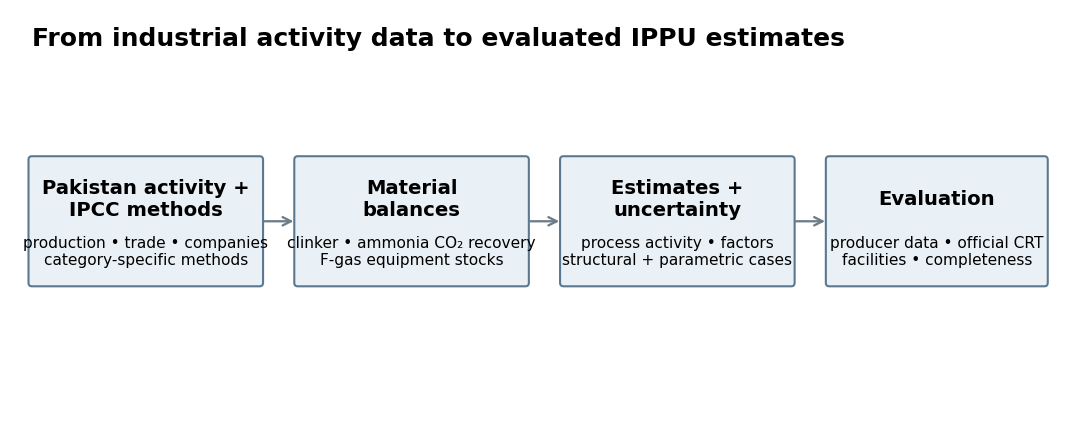
\includegraphics[width=0.94\textwidth]{ippu_framework.png}
\caption{Public inputs enter conserved material balances before category emissions are
calculated. Categories with insufficient evidence retain their notation keys and documented
data requirements.}
\label{fig:framework}
\end{figure*}

\subsection{Cement clinker balance}

For a fiscal year ending $y$, clinker contained in cement is
\begin{equation}
C^{\mathrm{cement}}_y=P^{\mathrm{cement}}_y f^{\mathrm{clinker}},
\end{equation}
and domestic clinker production is solved as
\begin{equation}
C^{\mathrm{production}}_y=C^{\mathrm{cement}}_y-I_y+X_y+\Delta S_y,
\label{eq:clinkerbalance}
\end{equation}
where $I$ and $X$ are clinker imports and exports and $\Delta S$ is the stock increase. This is
the sign convention implied by the IPCC Tier~1 worksheet: production plus imports minus
exports and stock increase equals clinker ground into cement \citep{ipcc2006ippu}. No public
stock series was identified, so $\Delta S=0$ in the reference configuration and stock change
remains an explicit data gap.

Process \COtwo{} is
\begin{equation}
E_{\COtwo{},y}=C^{\mathrm{production}}_y\,\mathrm{EF}_{\mathrm{clinker}},
\end{equation}
with an IPCC default factor of \SI{0.52}{\tonne} \COtwo{} per tonne of clinker. The estimate
covers calcination only. Kiln fuel belongs to Energy 1.A.2 and will be linked through the
shared facility inventory rather than included in 2.A.1.

\subsection{Structural and parametric uncertainty}

The source audit removes the apparent activity-source choice for FY2023--24: QIM and SBP agree
on \SI{39.566}{\mega\tonne}, while 48.011 Mt belongs to FY2021--22. Observed clinker trade is
required by Equation~\ref{eq:clinkerbalance} and is included in every valid current model.
The remaining declared structural choice is the clinker fraction, evaluated at 0.75 and 0.95.
Two no-trade calculations are retained separately as historical method benchmarks: one uses
the correct FY2023--24 activity to isolate trade omission, and the original result combines
trade omission with the superseded period tag. Neither enters the valid structural range.

Within both valid configurations, a seeded 10,000-iteration Monte Carlo samples bounded
triangular distributions for cement activity ($\pm5\%$), imports and exports ($\pm10\%$), and
the clinker factor ($\pm8\%$). The clinker fraction is fixed within each structural
configuration. We report conditional P2.5, median and P97.5 values rather than merging
discrete source/method choices into one probability interval.

For calendar 2022, the same equation is evaluated with twelve QIM monthly observations and
calendar-year clinker imports and exports. This makes the comparison with Pakistan's 2022 CRT
period-matched; the clinker fraction and zero stock change remain structural assumptions.

\subsection{Official-reporting audit}

The CRT audit extracts the native category cells rather than transcribing the published total.
For every numeric background row and gas, final emissions are reconstructed as
\begin{equation}
E^{\mathrm{final}}=A\times \mathrm{IEF}+R,
\end{equation}
where recovery $R$ is reported as a negative quantity. This treatment is important for
ammonia, where gross process \COtwo{} is partly recovered for downstream use. Arithmetic
closure tests the workbook; comparison with public evidence tests its activity, factor and
boundary choices.

\subsection{Spatial and temporal products}

The current cement provincial allocation preserves the legacy cement/limestone proxy only so
that downstream national and province tables remain reconciled. Its former Punjab activity
anchor is no longer treated as period-matched. Industrial
process emissions are point sources, so the target product is a facility ledger that
reconciles plant, district, province and national totals. Thirty-four facilities have been
identified; \num{24} carry resolved coordinates---one independently verified site geocode,
seven from named OSM industrial polygon centroids and \num{16} from the Global Energy
Monitor cement tracker, each point-in-polygon verified against
its census district at build---and the remaining \num{10} are located only to their reported
locality. Where both registers place the same works,
\texttt{outputs/ippu\_facility\_coordinate\_agreement.csv} records the separation: eight
sites are placed independently by OpenStreetMap and by the tracker and agree to within
\SIrange{0.024}{0.744}{\kilo\metre}. The file's other eleven rows are not evidence and say
so---those coordinates came from the tracker in the first place, so their distance to it is
zero and the comparison is a register against itself. Company-wide activity is assigned among plants only when
plant-specific evidence is available. Spatial and historical products are therefore reported
only where the required facility- or year-specific activity data have been assembled. A
1990--2024 coverage table records the remaining years as unavailable.

\section{Category Methods and Data Requirements}
\label{sec:factors}

The framework defines an IPCC calculation method and an evidence requirement for each
category. Higher-resolution activity data can therefore replace aggregate statistics without
changing the material balance or category definition.

\textbf{Mineral industries.} Cement uses Equation~\ref{eq:clinkerbalance}. Generic carbonate
methods are specified for lime, glass and other carbonate uses, but their Pakistan rows remain
NE until lime output by type, glass mass and type, cullet use and carbonate inputs are compiled.

\textbf{Chemical industries.} The ammonia ledger divides gross process \COtwo{} among
atmospheric emissions, recovery into urea, other recovery and permanent storage and asserts
zero residual. Nitric-acid emissions are estimated from production expressed as 100\% acid,
technology-specific
\NtwoO{} factors, the abated share, destruction efficiency and abatement utilisation. Total
fertiliser output or nameplate capacity alone is insufficient for either estimate.

\textbf{Metals and non-energy products.} QIM reports billet, ingot and lubricant production.
Iron and steel estimation additionally requires the production route and carbon inputs;
lubricant emissions require non-energy consumption and oxidation. These remaining inputs are
documented in the completeness matrix.

\textbf{Fluorinated gases.} A species-resolved equipment-bank model conserves annual chemical
supply across manufacturing loss, installed bank, operating leakage, retirement, recovery,
destruction and recovered gas available for reuse. AR5 and AR6 GWP registries include the HFC,
PFC, SF$_6$ and NF$_3$ species required by the CRT. The Ozone profile lacks the species- and
application-level data needed to estimate the bank, so 2.F remains NE in the independent
FY2023--24 inventory.

\FloatBarrier
\section{Evaluation Design}
\label{sec:validation}

Each evidence layer addresses a distinct question (Table~\ref{tab:evidence}).

\begin{table*}[htbp]
\centering
\footnotesize
\begin{tabular}{@{}p{0.30\linewidth}p{0.29\linewidth}p{0.30\linewidth}@{}}
\toprule
\textbf{Comparison} & \textbf{Purpose} & \textbf{Independence/limit} \\
\midrule
Clinker material closure & Physical accounting & Depends on cement fraction and zero stock change \\
QIM versus SBP fiscal series & Period and source audit & Independent official publications agree on FY2023--24 \\
Calendar-2022 cement versus CRT & Official method comparison & Matched year and category; clinker fraction remains assumed \\
Producer clinker versus Tier~1 & Independent activity/boundary evaluation & All sixteen producers report clinker; movements and stocks incomplete \\
CRT arithmetic reproduction & Spreadsheet QA & Tests arithmetic, not methodological validity \\
Ozone HFC consumption versus CRT & Completeness diagnostic & Consumption and annual emissions have different boundaries \\
Provincial proxy closure & Allocation QA & Reconciles exactly but is not spatial validation \\
\bottomrule
\end{tabular}
\caption{Evaluation roles. Agreement is interpreted only at the boundary supported by each
comparison.}
\label{tab:evidence}
\end{table*}

Automated quality-control tests verify clinker-balance closure, completeness of monthly trade
records, correct trade signs, inclusion of observed trade in current estimates, reproduction
of reported CRT activity--factor calculations and full 2.A--2.G coverage in the completeness
matrix. Provincial allocations must also reconcile exactly to the national total. Detailed
test definitions are provided in \ref{app:repro}.

The official comparison is category-specific. Pakistan's 2022 cement row is compared with an
independent calendar-2022 QIM/trade reconstruction under both clinker-fraction choices. The
official whole-IPPU total is not compared with the independently estimated cement component;
its category composition instead establishes the materiality of categories still missing from
the public-data estimate. Company clinker is an independent activity test, but not yet a
national Tier~2 result: every one of the sixteen producers now reports an exact clinker
quantity, but producer coverage, transfers and stocks have not been reconciled with QIM
cement production.

\section{Results}
\label{sec:results}

\subsection{The activity audit changes the reference calculation}

The apparent discrepancy in FY2023--24 cement activity results from an incorrect period
assignment. PBS QIM and the SBP
fiscal series both report \SI{39.566}{\mega\tonne}; the former
\SI{48.011}{\mega\tonne} statistic is the FY2021--22 value. The corrected reference therefore
contains \SI{29.6745}{\mega\tonne} of clinker at a 0.75 fraction. Adding
\SI{3.792074}{\mega\tonne} of exports and subtracting
\SI{0.026131}{\mega\tonne} of imports gives \SI{33.440443}{\mega\tonne} of inferred domestic
clinker production (Table~\ref{tab:balance}). At \SI{0.52}{\tonne\per\tonne}, process
emissions on that inferred route are \SI{17.389030}{\mega\tonne} \COtwo{}---the named
Tier~1 diagnostic. The reference does not use the inferred route: it takes the
\SI{41.953170}{\mega\tonne} of clinker the sixteen producers report and gives
\SI{21.815648}{\mega\tonne} \COtwo{} at the same factor.

\begin{table}[htbp]
\centering
\footnotesize
\begin{tabular}{@{}lrr@{}}
\toprule
\textbf{Clinker flow} & \textbf{Mt} & \textbf{Sign in inferred production} \\
\midrule
Clinker contained in cement & 29.674 & $+$ \\
Imports                     &  0.026 & $-$ \\
Exports                     &  3.792 & $+$ \\
Stock increase              &  0.000 & $+$ \\
\midrule
\textbf{Inferred domestic production} & \textbf{33.440} & \\
\bottomrule
\end{tabular}
\caption{FY2023--24 clinker balance. The zero stock row is explicit and unresolved.}
\label{tab:balance}
\end{table}

Using the correct FY2023--24 activity but omitting observed trade gives
\SI{15.430740}{\mega\tonne} \COtwo{}. Trade correction therefore adds 1.958 Mt, or 12.7\%,
and is a method correction rather than a valid structural alternative. The original
18.724 Mt result is retained only as a historical benchmark because it combines trade omission with the
misdated 48.011 Mt activity.

\subsection{Producer evidence against the two Tier~1 inferences}

All sixteen company filings sum to \SI{41.953170}{\mega\tonne} of actual clinker, equivalent
to \SI{21.815648}{\mega\tonne} \COtwo{} at the common factor---the reference activity. This
observed census is 125.5\% of the 0.75 Tier~1 inference and 101.4\% of the 0.95
inference---a near-identity that partly reflects the two constructions drawing on
overlapping reporting, and is therefore construction similarity as much as corroboration;
Fecto's quantity is read from its FY2025 annual report's comparative table
(Figure~\ref{fig:producers}). We use the reported census without extrapolation. If the company filings
and QIM cover the same producers and reporting period, and stock change is negligible, the
observed subset implies a diagnostic clinker fraction of 0.949. The low-clinker case is
therefore inconsistent with the company data unless the two sources differ in producer
coverage or reporting period, or unless clinker transfers and stock changes materially affect
the balance.

The company compilation constrains the national clinker balance but does not yet constitute a
complete Tier~2 activity dataset. A consistent set of opening and closing stocks, clinker
purchases, domestic sales, exports and clinker ground has not been reported. The unresolved
terms are documented without allocating the national residual among firms.

\begin{figure*}[htbp]
\centering
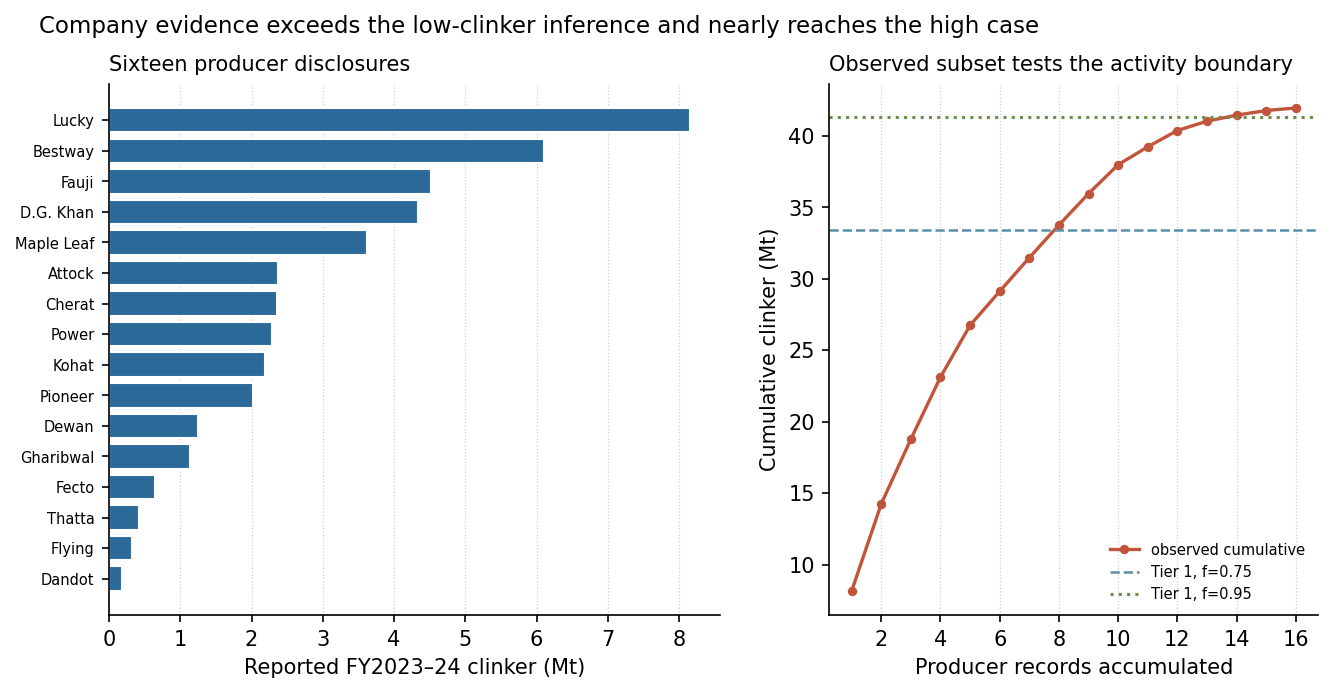
\includegraphics[width=0.98\textwidth]{ippu_producer_census.png}
\caption{Reported FY2023--24 clinker by producer (left) and the cumulative observed subset
against the two trade-corrected Tier~1 inferences (right). All sixteen census producers
report an exact quantity; Fecto's is the FY2024 comparative of its FY2025 annual report.}
\label{fig:producers}
\end{figure*}

\subsection{Valid cement models and conditional uncertainty}

With observed trade included in every current model, the structural range is
17.389--21.504 Mt \COtwo{} for clinker fractions of 0.75 and 0.95
(Figure~\ref{fig:cementevidence}); both ends of that range are priced against the
national total as named configurations in
\texttt{outputs/national\_configurations.csv}, and the observed census (21.816 Mt) sits
1.4\% above the high end. The reference Monte Carlo has a median of
\SI{21.809297}{\mega\tonne} and a 95\% interval of 20.227--23.452 Mt. The all-Portland
configuration has a median of 21.493 Mt and an interval of 19.937--23.062 Mt. The method
benchmarks are shown separately; the valid range is based exclusively on trade-corrected
models.

\begin{figure*}[htbp]
\centering
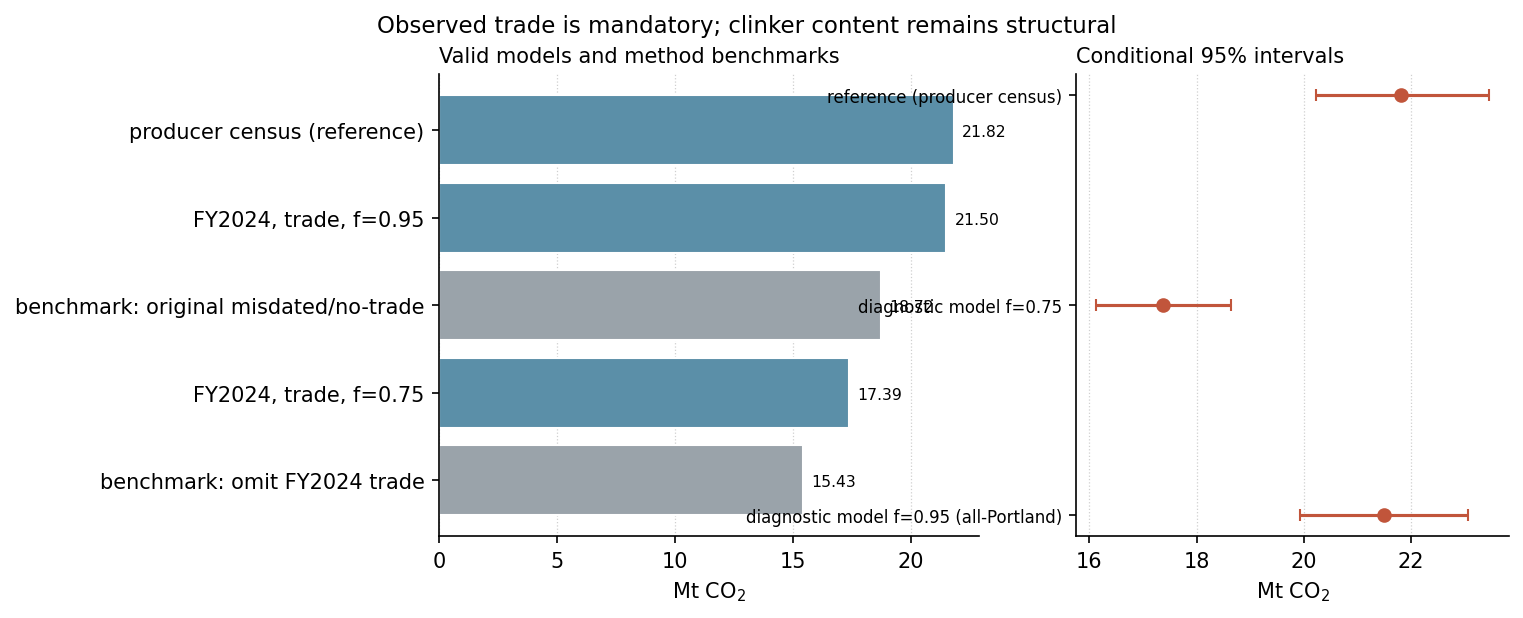
\includegraphics[width=0.98\textwidth]{ippu_cement_evidence.png}
\caption{Left: valid trade-corrected clinker-fraction models and separate method benchmarks.
Right: conditional parametric intervals within the two valid configurations.}
\label{fig:cementevidence}
\end{figure*}

\subsection{Calendar-2022 reconstruction sharpens the official comparison}

The 12 monthly QIM observations sum to \SI{44.331}{\mega\tonne} in calendar 2022. Combining
them with \SI{1.341580}{\mega\tonne} of clinker exports and
\SI{0.003999}{\mega\tonne} of imports gives \SI{34.585831}{\mega\tonne} of inferred clinker
and \SI{17.984632}{\mega\tonne} \COtwo{} at the 0.75 fraction. The 0.95 configuration gives
\SI{22.595056}{\mega\tonne}.

Pakistan's CRT cement row reports \SI{50.2455}{\mega\tonne} of activity and an implied factor
of 0.55539 t/t, yielding \SI{27.905848}{\mega\tonne} \COtwo{}. The independent matched-year
reconstructions are therefore 35.6\% and 19.0\% below the official result. The gap reflects
both activity (44.331 versus 50.246 Mt) and clinker/factor treatment; it is no longer an
artefact of comparing different years.

The CRT reports \SI{49.11203}{\mega\tonne} \COe{} for all IPPU in 2022. Mineral industries
account for 29.300 Mt and chemical industries 19.400 Mt; non-energy products and other
industrial processes contribute 0.217 and 0.192 Mt. All seven numeric background calculations
reproduce exactly, including the ammonia recovery term. The official discrepancy is therefore
methodological and empirical rather than spreadsheet arithmetic.

\begin{figure*}[htbp]
\centering
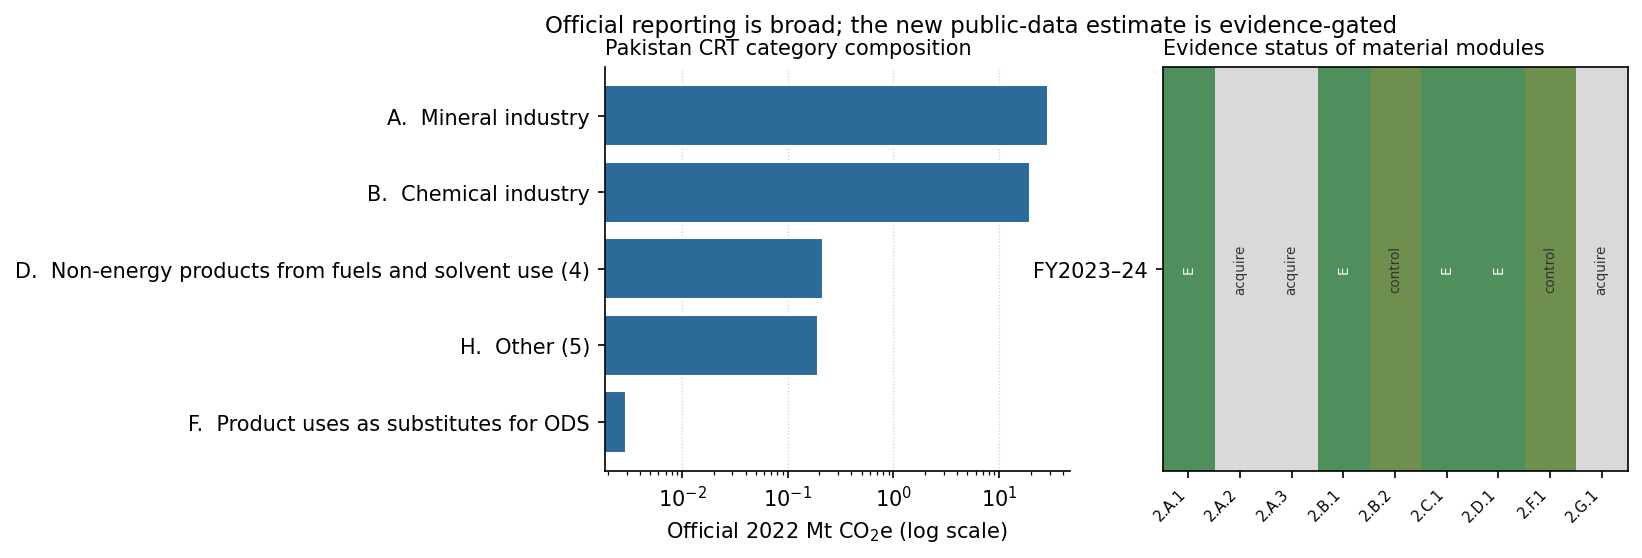
\includegraphics[width=0.92\textwidth]{ippu_official_audit.png}
\caption{Official 2022 IPPU category composition (left) and independent FY2023--24 evidence
status (right). Cement, ammonia, iron and steel and lubricant use are estimated; unsupported rows remain NE.}
\label{fig:official}
\end{figure*}

\subsection{Evidence available for the next categories}

Cement, ammonia, iron and steel, and lubricant use enter the FY2023--24 GHG module. Cement contributes \SI{21.816}{\mega\tonne} CO$_2$ to the \SI{25.535}{\mega\tonne} module total; the following plant evidence identifies remaining process and Tier~2 gaps rather than implying ammonia is wholly absent. One ammonia plant reports
\SI{0.311242}{\mega\tonne} of output in 2024, and historical plant and CDM records identify
nitric-acid technology and abatement projects. National estimates require complete plant
coverage, recovered \COtwo{} and annual abatement operation. For ammonia the generated
reconciliation now compares four independent activity pathways and locates the
inconsistency: the official 2022 filing's \SI{11467}{\kilo\tonne} of ammonia would require
roughly half again more gas than the whole fertiliser sector draws, embodied ammonia in
NFDC's product-wise production sits near \SI{4500}{\kilo\tonne}, and the quantifiable plant
floor is \SI{548}{\kilo\tonne} from two of eight census plants. The filing's recovery term,
by contrast, implies \SI{6442}{\kilo\tonne} of urea, consistent with audited production;
the suspect leg is the activity, not the recovery. The HFC evidence similarly
requires species- and application-specific equipment data before consumption can be related to
annual emissions.

Chemical observations are reported separately by year, and verified CDM reductions are
assigned only to their stated monitoring periods. For Pakarab, the available evidence includes
line-level production, operating days and abatement technology for 2008.

Cement has the most detailed company-level production support. Ammonia retains product-derived output and recovery assumptions; nitric acid still lacks complete own-year production and demonstrated abatement operation. The primary geographic product preserves company-level uncertainty and licence-compatible locations, with unsupported placement retained in the unallocated account.

\subsection{Air-pollutant process coverage}
The admitted air classes estimate ammonia-process releases, electric-route steel emissions and soda-ash process emissions with their specific factors and physical activities. Cement air factors cover an integrated kiln stack and are accounted once under industry; cement GHG calcination remains separate from kiln fuel. Urea finishing, nitric-acid pollutants, lime, glass and other unresolved processes remain explicit coverage gaps. Missing species are not filled with zero or with an uncontrolled screening endpoint.

\section{Discussion}
\label{sec:discussion}

\subsection{Trade correction is part of the method}

Pakistan's net clinker exports are 12.7\% of the correctly period-tagged no-trade estimate
after conversion to \COtwo{}. Omitting them assigns calcination to the country where exported
clinker is ground rather than the country where it was produced. The corrected equation
therefore changes both the magnitude and the geographic boundary of 2.A.1. Stock movement
remains unresolved, but it is now visible as one term in the same physical balance.

The source audit also illustrates why period and source documentation are part of the
calculation. The reported 48.011 and 39.566 Mt values were consecutive observations in the
same official fiscal series, rather than competing estimates for one year. Correcting the
period changes the headline result more than the remaining parametric uncertainty and removes
a spurious structural choice.

\subsection{A complete sector starts with completeness accounting}

Pakistan's official results make the scope problem concrete. In 2022, chemical-industry
emissions were two-thirds as large as mineral-industry emissions. A cement calculation can
therefore be rigorous without representing the full IPPU sector. The framework avoids
conflating the two by assessing the evidence and method available for every 2.A--2.G category
before calculating a sector total.

This design also changes how public data are interpreted. A soda-ash production record is
useful for 2.B.7 only after the production route is known and must be distinguished from
soda-ash consumption under mineral uses. Total fertiliser output cannot estimate ammonia,
where process \COtwo{} recovery into urea is central. Billets identify steel output but not
the production route or carbon inputs. HFC consumption establishes chemical supply, whereas
annual emissions depend on equipment stocks and leakage. These distinctions preserve the
physical meaning of each category estimate.

\subsection{The CRT audit identifies immediate empirical priorities}

All tested CRT rows reproduce exactly from their reported activities, implied factors and
recovery terms. Its \SI{49.112}{\mega\tonne} result is consequently traceable to reported
activities, factors, recovery and omissions rather than a spreadsheet mistake. Three
empirical priorities follow.

First, the sixteen-company clinker census---complete for production since Fecto's exact
output was read from its annual report---should be completed with clinker purchases, sales
and stocks. The census already exceeds the low-clinker inference and slightly exceeds the
high case, so these data must reconcile reporting boundaries as well as replace Tier~1
activity. Second, plant ammonia and nitric-acid records can
reconstruct the official chemical-industry result while preserving recovered carbon and
abatement. Third, species- and application-level HFC imports, exports and equipment stocks can
support an estimate based on the Ozone consumption data. The small HFC value in the 2022 CRT
and the much larger consumption statistic have different accounting boundaries, but together
they make product-use completeness a high-priority audit. The CRT entry is smaller than
``small'' conveys and its shape matters: all of category~2.F is a single species, HFC-23,
entered at \SI{0.236955}{\tonne} as exactly \SI{1}{\percent} of a declared
\SI{23.69549}{\tonne} operating stock and filed under sub-category 2.F.1.a commercial
refrigeration, with every other species and sub-category \texttt{NE} or \texttt{NO}.
HFC-23 is an HCFC-22 by-product and a cascade low-temperature refrigerant rather than a
commercial refrigerant, so the species assignment is a reporting artefact, and Pakistan's
first Biennial Transparency Report then books 2.F, 2.C, 2.E and 2.G all at zero. The two
most recent official submissions therefore disagree about whether the category exists,
which is not a boundary difference.

The leak rate is the other decision that is easy to overlook, and
\texttt{outputs/pakemis\_fgas\_leak\_rate\_adjudication.csv} prices it. The
species-resolved bank applies one operating loss fraction per stratum---refrigeration
\SI{8}{\percent} per year, stationary air-conditioning \SI{6}{\percent}, mobile
air-conditioning \SI{15}{\percent}---while IPCC Table~7.9 publishes a rate for each
sub-application. Mobile air-conditioning maps one-to-one onto its table row and needs no
weighting. Stationary air-conditioning lumps chillers with residential and commercial
units, whose bands overlap, and \SI{6}{\percent} is admissible for either part.
Refrigeration lumps five sub-applications whose operation-emission bands span
\SIrange{0.1}{50}{\percent} per year with no common value, and the single
\SI{8}{\percent} lies outside two of them, from \num{16} to \num{80} times above
domestic refrigeration's whole band. For that part the rate is not uncertain but inadmissible, and
the split that would resolve it is not held.

What the envelope shows is that the rate decides timing rather than mass. Re-running the
bank across refrigeration's full band moves the operating channel from
\SI{0.013}{\mega\tonne} to \SI{2.062}{\mega\tonne} of \COtwo e, a factor of
one hundred and fifty-five, while the stratum total moves only
\SIrange{0.757}{2.192}{\mega\tonne}: gas the operating channel does not leak is still
emitted at retirement, because no recovery is credited anywhere. The deferred mass appears
instead as a closing bank of \SIrange{1.959}{12.559}{\mega\tonne} of \COtwo e. A low
leak rate is therefore not a smaller inventory but a larger future liability, and
category~2.F contributes zero to every reported total throughout.

\subsection{Facility geography is preferable to proxy geography}

The current provincial cement allocation is retained for compatibility with the national
inventory, but its earlier Punjab activity anchor is not period-matched. Cement kilns,
ammonia plants, nitric-acid plants, soda-ash works, steel mills and glass plants are point
sources. A shared facility inventory can assign process emissions to their physical sites and
link the same installation to Energy 1.A.2 combustion without mixing the two categories.
Diffuse product use, especially refrigeration and air-conditioning, can then be represented
through equipment stocks and population or service activity rather than an industrial point
proxy.

\subsection{The matched official comparison reveals a second cement discrepancy}

Calendar matching does not close the official cement row. Even the 0.95 public-data
configuration remains 19\% below the CRT, while the low-clinker model is 36\% below. Part of
the difference is visible in the activity data: the CRT uses 50.246 Mt against 44.331 Mt from
the monthly QIM reconstruction. The remainder is embedded in the CRT's 0.55539 t/t implied
factor and any clinker, stock or coverage treatment behind it. Because the workbook arithmetic
closes, resolving this difference requires the institutional derivation and company clinker
balance rather than further arithmetic verification.

\subsection{Transferability}

The framework is transferable because its accounting structure is independent of any one
national data source. Countries with incomplete industrial statistics commonly combine
national production totals, trade data, partial company reporting, ozone-substitute
consumption records and official inventory submissions. Higher-quality evidence can replace
aggregate activity assumptions without changing the material balances or category
definitions. Exact mass closure, category completeness and an auditable official crosswalk
remain valid as the quality of the underlying evidence improves.

\section{Limitations}
\label{sec:limitations}

The independent FY2023--24 estimate covers four IPPU categories: cement calcination
(2.A.1, \SI{21.815648}{\mega\tonne}), ammonia production (2.B.1, \SI{3.2433}{\mega\tonne}),
iron and steel (2.C.1, \SI{0.3931}{\mega\tonne}) and lubricant use (2.D.1,
\SI{0.0833}{\mega\tonne}), for a module total of \SI{25.5354}{\mega\tonne} of \COtwo{}.
Methods and data requirements are defined for the categories that remain unestimated --- lime
(2.A.2), glass (2.A.3), nitric acid (2.B.2), HFCs (2.F) and SF$_6$ (2.G) --- and those stay
NE until the required activity and process data are available. Cement is therefore
\SI{85.4}{\percent} of the module rather than all of it: the
\SI{21.815648}{\mega\tonne} figure represents cement-process \COtwo{} rather than total
IPPU or total cement emissions, and the \SI{17.389}{\mega\tonne} Tier~1 inference at the 0.75
clinker fraction is a named diagnostic beside it, not the reference.

National clinker production is observed at the company grain; stock change is not. All sixteen
producer records together exceed the low-clinker inference by a quarter and the high case by
1.4\%, but the company-level purchase, sale, grinding, export and stock fields remain
missing. The company compilation therefore constrains the national clinker balance but does
not yet constitute a complete Tier~2 activity dataset.

The conditional Monte Carlo covers activity, trade and factor ranges within each clinker-
fraction model. It does not assign a probability to the 0.75 or 0.95 configuration. Stock
uncertainty is not sampled because no defensible public bound was identified.

The matched calendar-2022 comparison still depends on an assumed clinker fraction and zero
stock change. It demonstrates that year mismatch does not explain the difference from the CRT,
but it cannot reconstruct the official institutional derivation without its internal clinker
and coverage evidence.

The chemical plant table is partial. Nameplate capacity, one calendar-2024 ammonia observation and CDM
project existence cannot substitute for national plant production, recovered \COtwo{} or
annual abatement operation. Ozone-profile HFC consumption provides a national supply statistic
but cannot be compared directly with annual emissions.

Company-level clinker production does not establish plant-level output. Facility-assisted geography uses only the source locations compatible with the primary package's licence; ODbL-derived alternatives remain separate. Unsupported or excluded locations remain unallocated rather than inheriting another source's coordinates.

The common annual core covers ten fiscal years, July 2015--June 2025. The reference-year company analysis does not imply observed annual plant geography. Soda ash production is observed; its Solvay-route GHG treatment places the coke combustion term under Energy, where missing coke activity remains explicit. The IPPU notation must not be read as evidence that soda ash production does not occur. The admitted soda-ash air process class has its own factor and boundary. Lime, glass, nitric acid and fluorinated-gas emissions remain unresolved where required process or equipment data are missing.

\section{Conclusion}
\label{sec:conclusion}

This study establishes an IPPU-wide accounting framework for Pakistan while independently
estimating cement calcination as its first category. Every 2.A--2.G category is assessed,
industrial material balances are conserved and official reporting is extracted at cell level.
Categories lacking sufficient evidence remain explicitly unestimated, with their remaining
data requirements identified.

The first module has changed in three material ways. The source audit establishes that
\SI{48.011}{\mega\tonne} is FY2021--22 cement output and that the FY2023--24 reference is
\SI{39.566}{\mega\tonne}. Applying observed clinker trade to that activity gives
\SI{17.389}{\mega\tonne} \COtwo{} at a 0.75 clinker fraction, compared with 15.431 Mt when
trade is incorrectly omitted. The Tier~1 configurations span 17.389--21.504 Mt across the
two IPCC clinker-fraction cases---0.75 at the low end, 0.95 at the high---and the span is a
structural benchmark range, not a number with a preferred point. The reference is not on
it: since rc30 it is the producer census's own disclosed clinker, \SI{21.816}{\mega\tonne}
\COtwo{} (conditional 95\% interval 20.227--23.452 Mt), 1.4\% above the high case, and the
0.75-fraction model is priced beside it as the \emph{cement\_tier1\_model\_low}
configuration. Earlier editions of this paragraph called the low case the reference and
mislabelled the span's ends.

All sixteen producer filings now disclose actual clinker---\SI{41.953}{\mega\tonne},
125.5\% of the low-clinker model inference and 101.4\% of the high case, with Fecto's
\SI{651048}{\tonne} read from its FY2025 annual report's comparative table rather than
imputed from capacity---and since rc30 that census IS the reference activity, with the
Tier~1 model beside it as the named diagnostic. What remains for the movement ledger is
the material balance: stocks, transfers and clinker ground, the Tier-2 fields no filing
publishes.

The matched calendar-2022 reconstruction gives 17.985--22.595 Mt, below the official cement
row of \SI{27.906}{\mega\tonne}. Pakistan's full CRT reports
\SI{49.112}{\mega\tonne} \COe{}, including \SI{19.400}{\mega\tonne} from chemicals. The next
empirical priorities are consequently bounded: finish clinker production and movements;
complete plant ammonia/nitric-acid production, recovery and abatement; and compile the
species- and application-level data required for an HFC equipment-bank model.

The current empirical estimate remains limited to cement calcination, while the same framework
provides defined pathways for independent ammonia, nitric-acid and fluorinated-gas estimates
as the required plant- and application-level data become available.

\FloatBarrier

\section*{Code and data availability}
The calculation code, activity data and generated outputs are version-controlled in the
inventory repository (\url{https://github.com/RehanAhmad13/pakistan-emissions-sectors}) and reproduce
from the commands in \ref{app:repro}. Numerical results are read from generated CSV
files, with automated checks confirming agreement between the manuscript and calculations.

\bibliographystyle{elsarticle-harv}
\bibliography{../../paper_common/references}

\appendix
\renewcommand{\thetable}{\arabic{table}}%
\renewcommand{\thefigure}{\arabic{figure}}%
\section{Reproduction and generated outputs}
\label{app:repro}

\begin{verbatim}
pip install -e .
python3 -m pkinv.sectors.ippu.run_ippu
python3 -m unittest discover tests
python3 -m pkinv.report.figures
python3 scripts/sync_figures.py
\end{verbatim}

The run generates the sector's headline tables---\texttt{ippu\_totals\_2024.csv} (the result by
category in both common-GWP vintages), \texttt{ippu\_by\_stream\_2024.csv} (category, subitem
and gas in gigagrams with each row's uncertainty, activity year and period kind,
evidence class, temporal and spatial method and source), \texttt{ippu\_provincial\_2024.csv}
(the province-level AR5 total, each row carrying the allocation status that produced it) and
\texttt{ippu\_monthly\_2024.csv} (the twelve-month layer with each month's share, the emissions
it implies and the basis of the shape)---together with the evidence tables below. Each is
named, because a reader reproducing the run is otherwise told what it produces without being
able to tell which file is which; every quantity this paper prints from one of them is checked
against it by the verification registry.

\begin{description}\itemsep2pt
\item[\texttt{ippu\_cement\_material\_balance\_2024.csv}] the clinker material balance:
  domestic production, trade and stock terms against inferred clinker.
\item[\texttt{ippu\_cement\_producer\_census\_2024.csv}] the \num{16}-company producer
  census, each entity's reported clinker quantity (Section~\ref{sec:data}).
\item[\texttt{ippu\_company\_clinker\_2024.csv}] company-level clinker flows for the same
  \num{16} entities.
\item[\texttt{ippu\_company\_clinker\_coverage\_2024.csv}] the company-against-census
  coverage reconciliation---identical universe and period, zero stock change.
\item[\texttt{ippu\_cement\_valid\_structural\_2024.csv}] the valid trade-corrected
  structural models: scenario, cement source, clinker fraction and resulting \COtwo{}.
\item[\texttt{ippu\_cement\_tier\_comparison\_2024.csv}] the same estimate by method and
  coverage, the producer census as reference.
\item[\texttt{ippu\_cement\_method\_benchmarks\_2024.csv}] the two retained no-trade
  benchmarks, marked screening-only, isolating the bias from omitting observed clinker trade.
\item[\texttt{ippu\_cement\_conditional\_intervals\_2024.csv}] conditional Monte Carlo
  intervals per configuration, with the deterministic value, the quantiles, the draw count and
  the seed.
\item[\texttt{ippu\_cement\_matched\_calendar\_2022.csv}] the matched calendar-2022
  reconstruction, inferring clinker production from that year's own activity and trade.
\item[\texttt{ippu\_cement\_activity\_reconciliation.csv}] a reported cement quantity
  against the period it actually belongs to, retained so a superseded period tag cannot
  re-enter as a structural alternative.
\item[\texttt{ippu\_ammonia\_activity\_reconciliation.csv}] ammonia activity by pathway
  against the official filing, with each pathway's independence from it recorded.
\item[\texttt{ippu\_fertilizer\_gas\_cross\_source\_2024.csv}] the fertiliser gas
  cross-source check: NFDC plant meters against the gas ledger, with the feed and fuel shares
  and their agreement.
\item[\texttt{ippu\_chemical\_plant\_activity.csv}] the chemical-plant evidence table
  (Section~\ref{sec:limitations} states what it does not cover).
\item[\texttt{ippu\_activity\_controls\_2024.csv}] the activity controls, one row per IPCC
  code and product, each with its source reference, coverage and data tier.
\item[\texttt{ippu\_facility\_registry.csv}] the facility registry and
  \texttt{ippu\_facility\_coverage.csv} its geocoding coverage by district---declared,
  geocoded and ungeocoded counts (Section~\ref{sec:data}).
\end{description}

The run also writes the CRT activity--factor bridge, the full completeness matrix, nitric-acid
evidence, HFC data specifications, the source manifest, the CRT cell extraction, the
quality-control report and the run manifest.

The run manifest records every input hash, output name, reference result and structural range.
The CRT cell audit additionally records the source ZIP and workbook hashes, worksheet, cell,
raw value, formula and cell-value hash. The generated national total contains only the
independently estimated 2.A.1 process \COtwo{} component.

\section{Completeness and data requirements}

Each detailed category is documented in \texttt{ippu\_completeness\_2024.csv} by IPCC code,
gas, notation key, activity and method status, public source, available years, source role,
materiality and remaining data requirement---the table this section has always described and
never named. The gas split behind the fertiliser feedstock is published beside it in
\texttt{ippu\_\allowbreak fertilizer\_\allowbreak gas\_\allowbreak monthly\_\allowbreak 2024.csv}, which carries feed and fuel
volumes in million cubic feet by month with each month's share of the year and the feedstock share it
implies. The highest-priority data needs are:

\begin{enumerate}[leftmargin=*]
\item APCMA and cement producers: clinker production, purchases, sales, trade and stocks;
\item NFDC and fertiliser producers: ammonia and 100\%-nitric-acid output, feedstock, recovered
      \COtwo{}, process technology and \NtwoO{} abatement;
\item National Ozone Unit and Customs: annual chemical/application imports, exports,
      destruction and equipment charge for HFCs;
\item PBS and industrial producers: marketed and captive lime, glass tonnes/type/cullet,
      carbonate inputs, steel route and carbon inputs, and lubricant consumption;
\item NTDC, distribution companies and major equipment owners: SF$_6$ equipment, purchases,
      refills, recovery and retirement.
\end{enumerate}

\section{Source hierarchy}

Methods and cement factors are from IPCC Volume~3 \citep{ipcc2006ippu}. FY2023--24 cement
activity is from PBS QIM \citep{pbsqim2024} and is corroborated by the SBP fiscal series
\citep{sbpstatsupp2024}; that cross-check corrects the former Pocket Book period tag.
FY2023--24 clinker trade is from UN Comtrade \citep{uncomtrade2024clinker}, and calendar-2022
trade is cross-checked through WITS/UN Comtrade \citep{witsclinker2022}; company clinker
sources are recorded row by row in the producer ledger.
The official comparison is Pakistan's 2022 CRT
\citep{pakcrt2026}, and HFC consumption data are from the Ozone Secretariat country profile
\citep{pakistanozoneprofile}.


\end{document}
